\documentclass[russian,utf8,a1paper,nostitching,simple]{eskdgraph}
\usepackage[T2A]{fontenc}
\usepackage{pscyr}
\usepackage{tikz}
\usepackage{color}

\newcommand{\No}{\textnumero}

\ESKDunitName{Структура приложения}
\ESKDsignature{ГУИР.000000.001 ПЛ}
\ESKDletter{}{Т}{}
\ESKDauthor{Будный}
\ESKDchecker{Лаппо}
\ESKDcolumnXIfIII{\color{red}{???}}
\ESKDnormContr{Протченко}
\ESKDapprovedBy{Навроцкий}
\ESKDgroup{ИТАС, гр. 120602}

\begin{document}

\ESKDthisStyle{empty}
\begin{ESKDdrawing}
  \centering
  {\fontsize{50}{60}\selectfont Структура приложения}

  \vspace{2cm}
  % \vline
  % \hline
  \begin{minipage}{38cm}
    \centering
    \ESKDfontX{Преценденты использования} \\
    \vspace{2cm}
    \centering
    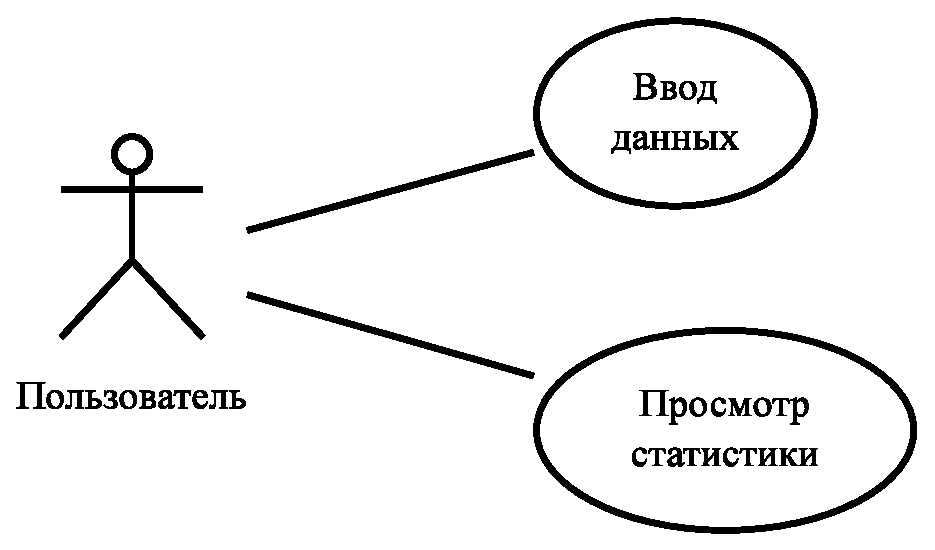
\includegraphics[height=15cm]{fig/design_use_cases.eps}

    \vspace{4cm}
    \centering
    \ESKDfontX{Экраны приложения} \\
    \vspace{2cm}
    \centering
    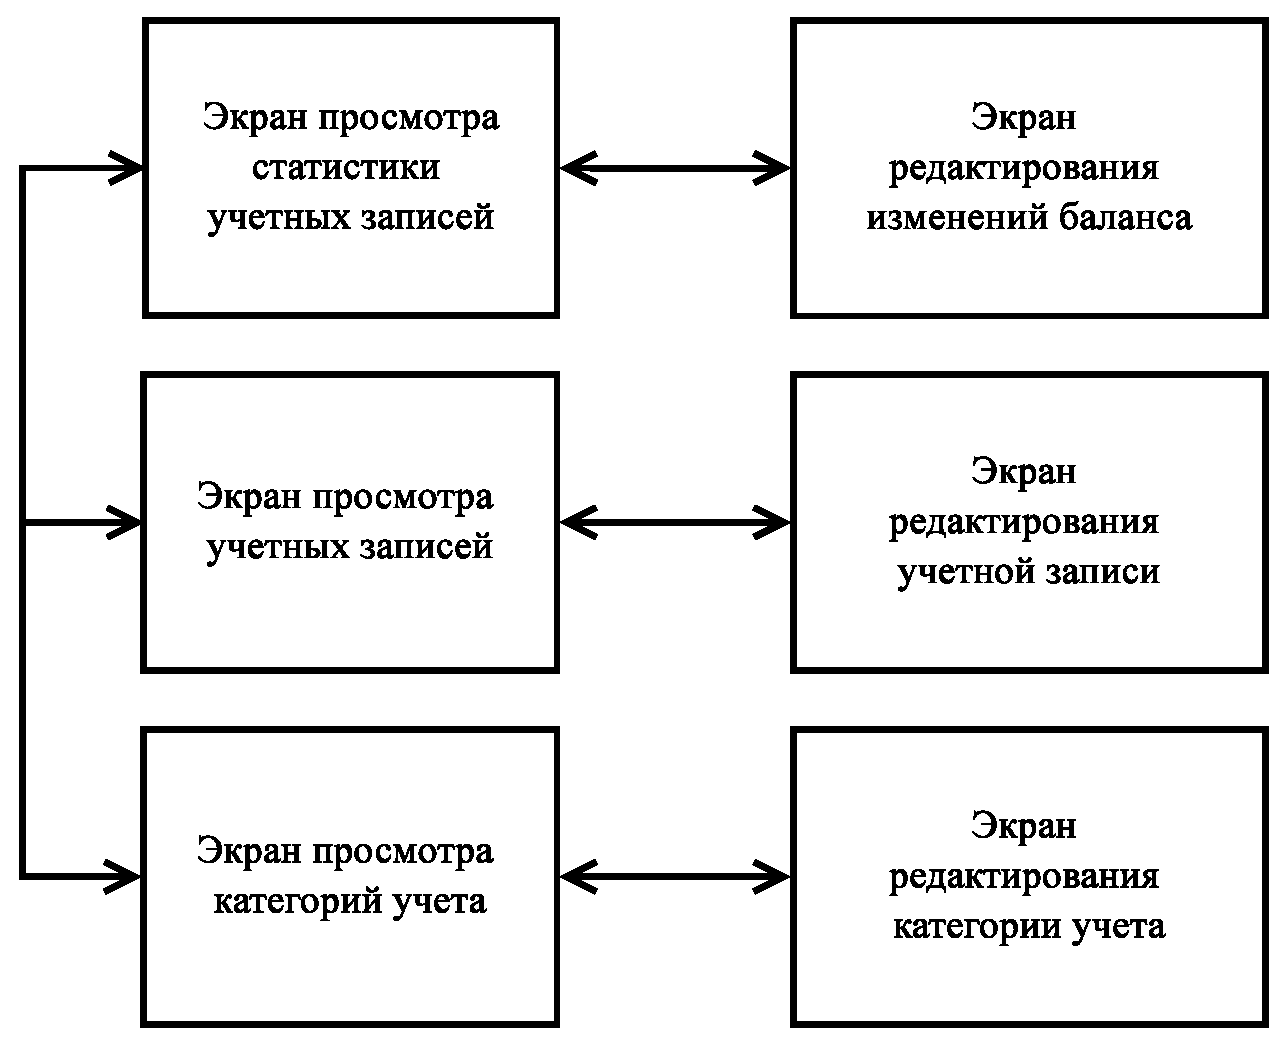
\includegraphics[height=25cm]{fig/design_activities.eps}
  \end{minipage}
  % \vline
  \hspace{2cm}
  % \vline
  \begin{minipage}{42cm}
    \centering
    \ESKDfontX{Паттерн MVP} \\
    \vspace{2cm}
    \centering
    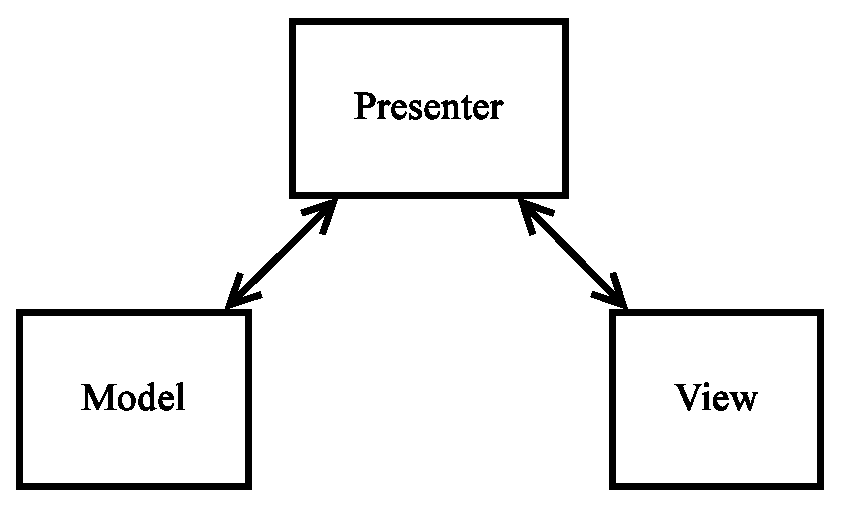
\includegraphics[height=15cm]{fig/design_mvp.eps}

    \vspace{4cm}
    \centering
    \ESKDfontX{Подсистемы приложения} \\
    \vspace{2cm}
    \centering
    \includegraphics[height=25cm]{fig/design_main.eps}
  \end{minipage}
  % \vline
  % \hline
\end{ESKDdrawing}

\setcounter{page}{1}
\ESKDthisStyle{formI}
\begin{ESKDdrawing}
\end{ESKDdrawing}

\end{document}
